\documentclass[11pt,a4paper]{article}
\usepackage[a4paper, twoside=false, tmargin=2.5cm, bmargin=2.5cm, inner=2.5cm, outer=2.5cm]{geometry}
\usepackage[utf8]{inputenc}
\usepackage[T1]{fontenc}
\usepackage[english]{babel}
\usepackage[english]{varioref}
\usepackage{graphicx, float, caption, subfig, amsmath, amssymb, mathrsfs}
\usepackage{blindtext}
\usepackage{scrextend}

\usepackage{array, booktabs, caption}
\usepackage{adjustbox}
\usepackage{multirow}

\usepackage{makecell}
\renewcommand\theadfont{\bfseries}
\usepackage{caption}
\usepackage{subcaption}
\usepackage{wrapfig}


\title{MOOC Visualisation}
\author{Frédéric \textsc{Moret}}

\makeatletter 
\AtBeginDocument{\markboth{\@author}{\@title}} 
\AtBeginDocument{\renewcommand{\labelitemi}{-}}

\pagestyle{headings}

%%% BEGIN DOCUMENT
\begin{document}

%TITLE
\begin{titlepage}
\begin{center}

{\Large \textsc{Communication Systems}}\\\medskip
{\Large \textsc{Optional Semester Project}}\\\medskip
{\Large Master Semester 4 - Spring 2017}\\\vspace{4cm}

{\Huge \@title}\\\vspace{4cm}

\begin{tabular}{ll}
{\Large \textit{Student:}}   & {\Large \@author} \\  & \\
{\Large \textit{Supervised by:}}
& {\Large Prof. Patrick \textsc{Jermann}}  \\ 
& {\Large Dr. Francisco \textsc{Pinto}} 
\end{tabular}
\vspace{3.5cm}

{\Large \@date}\vspace{3cm}

{\Large \textsc{Centre pour l'éducation à l'ère digitale}}\\\medskip
{\Large \textsc{EPFL}}\\\vspace{7mm}

\includegraphics[width=4cm]{pictures/epfl.png}

\end{center}
\end{titlepage}
%END TITLE

\newpage

\tableofcontents

\newpage

\pagenumbering{arabic}

\setcounter{page}{1}

\section{Introduction}

In the last 10 years, the "Massive Open Online Courses" (also known as MOOCs) have grown exponentially. With the expansion of the internet access around the globe, it became the easiest way to provide education in less developed areas, in particular in Africa. \\
\\
This growth was both in term of users, and in term of content. A lot of universities have begun to record MOOCs, and (for a large majority of them) have released them for free. \\
\\
Our university, the EPFL (Ecole Polytechnique Fédérale de Lausanne) has followed the trend, and has now a large collection of those courses available. \\
\\
With all those courses comes of course a lot of users data, as the behavior of users has been recorded. For now, this data is not used. The goal of this project is to analyse this data, and to extract the more important hints and conclusions, in order to create a tool for teachers. This tool has to be as intuitive as possible, to ensure that teachers reviewing their previous courses will be able to locate problems / advantages of them very easily. \\
\\
The project consists in two different parts. First, we process the data, and then we create a visualization for it. We will explain in details both processes, as well as the ideas / problems we encountered.

\section{Data Analysis} \label{data_analysis}

In this section, we will summary the pipeline we used. 

\subsection{Data Origin}

All the MOOCs at EPFL are hosted on one of two different MOOCs platforms, either on Coursera \cite{coursera} or EDX \cite{edx}. Thus, we had to be sure that the data coming from those two different sources had enough similarities, or equivalences, to be used. \\
\\
The logs available for those two platforms are almost identical, except for the fact that Coursera only identifies users by SessionID instead of AccountID, which means that a user who watches a video twice and log out/in in-between will be considered as two different persons by Coursera, while as the same person by EDX. \\
\\
After doing a few tests, this does not impact the data in general, so we can consider both sources to be reliable. \\
\\
EDX also provides Data on another form, mainly the number of unique users and the number of total viewers for each 5-seconds chunk of a video. As they already display thoses statistics visually on their dashboard, we've decided not to use them, and to stick to the logs. This allows us to provide the same output for both Coursera and EDX courses. \\
\\
For section \ref{data_analysis}, we'll use data from one specific video, Week 7 part 4 of Course BIO-465. It is hosted on EDX. All the plots represent Data from this video.

\newpage

\subsection{Raw Data}

The Data we get from Coursera and EDX is structured as follow. Each entry has the following fields. \\
\begin{align*}
\begin{array}{|c|c|c|c|c|c|c|}
\hline
\text{UserID} & \text{TimeStamp} & \text{EventType} & \text{CurrentTime} & \text{OldTime} & \text{NewTime} & \text{NewSpeed}\\
\hline
\end{array}
\end{align*}

\begin{labeling}{OldTime/NewTime}
    \item [UserID] This field is - as mentioned above - either an AccountUserID (for EDX Data) or a SessionUserID (for Coursera Data). As the Data has been anonymized, it's a number.
    \item [TimeStamp] This field represents the exact time at which the event has occurred. (it's a number, representing seconds between the beginning of Unix time (01.01.1970 at 00:00) and the time of the event).
    \item [EventType] This field corresponds to the type of event logged. It is one of six different types. They will be discussed in a the following section.
    \item [CurrentTime] This field is used only by two events, Video.Play and Video.Pause. It represents the time of the video at which the event has occurred (up to 1 millisecond precision).
    \item [OldTime/NewTime] Those two fields are used only by Video.Seek events. They represent the source and the target times of the video.
    \item [NewSpeed] This one is only used by Video.SpeedChange. It represents the new speed of the video.
\end{labeling}

\subsection{Data Selection}

As mentioned above, the Data is separated between six different events. The "Nbr" field represents the number of occurrences of each event in our video.\\
\\
\begin{tabular}{|c|c|c|c|c|}
\hline
\thead{EventType} & \thead{Analyzed} & \thead{Final \\ Version} & \thead{Comments} &  \thead{Nbr} \\
\hline
Video.Pause & \multirow{2}{*}{Yes} & \multirow{2}{*}{No} & \multirow{2}{*}{\makecell{
Those two events come together. \\
We will discuss them in a further section.}} & 370 \\
\cline{1-1} \cline{5-5}
Video.Play & & & &  562\\
\hline
\multirow{2}{*}{Video.SpeedChange} & \multirow{2}{*}{No} & \multirow{2}{*}{No} & \multirow{2}{*}{\makecell{Not enough Data, only a few users \\
actually change the speed of a video.}} & \multirow{2}{*}{2}\\
 & & & &  \\
\hline
\multirow{5}{*}{Video.Seek} & \multirow{5}{*}{Yes} & \multirow{5}{*}{Yes} & 
\multirow{5}{*}{\makecell{This event is the most popular one. We've \\
decided to use it exclusively, because of \\
the amount of information contained it in.\\
We will explain later in details what can \\
be decuct from it, and why.}} & \multirow{5}{*}{347}\\
 & & & & \\
 & & & & \\
 & & & & \\
 & & & & \\  
\hline
\multirow{2}{*}{Video.Load} & \multirow{4}{*}{No} & \multirow{4}{*}{No} & 
\multirow{4}{*}{\makecell{Those two events are quite irrelevant to \\
our analysis, as they only occurred when \\
the user launches the video, and when he \\
selects the potential subtitles.}}& \multirow{2}{*}{513} \\
 & & & & \\
\cline{1-1} \cline{5-5}
\multirow{2}{*}{Video.Transcript} & & & & \multirow{2}{*}{508}  \\
 & & & & \\
\hline
\end{tabular}


\subsection{Data Cleaning}

Once all the Data was acknowledged, we had to clean it. As we decided to only work with Pauses, Plays and Seeks, the following subsections will explain how we cleaned it.


\subsubsection{Events : Pauses \& Plays}

Those two events could be really useful, as the number of occurrences is quite high. Nevertheless, the problem is that the Data is really noisy. We've decided to merge them into a single event, with a few constraints. \\
The time difference between the pause and the subsequent play should not exceed 10 minutes. This constraint is meant to eliminate pauses unrelated to comprehension, for example dealing with real-life problems, or social ones. \\
It also has to be greater than 10 seconds. We estimated that pausing the video for less than 10 seconds won't help for the comprehension, therefore those events are irrelevant.\\
\\
After cleaning the Data with those rules, we obtain only 81 events, which represents around $20\%$ of the initial Data Set. \\
\\
We will discuss later how good and usable are those results.

\subsubsection{Events : Seeks}

The Video.Seek events are the most powerful in term of information. To understand why, we need to compare the Pause/Play event with this one. When a user stops the video at a certain time, and plays the video again after a while, it means that he had some problems to understand the content of this specific part of the video. When a user seeks to a specific time of the video, he wants to go back to this part, or to skip something to arrive at this exact time. Therefore, instead of having only the information of the time of pause, we also have the information about the source of the user, it adds a new dimension to the information. \\
\\
This information allows us to display a two-dimensional graph instead of a simple bar graph. Nevertheless, it is possible that the results for the Pauses\&Plays event are similar to the Seek event ones. We will detailed the comparison later. \\
\\
Similarly to the Pauses\&Plays, the Data is really noisy. If a user is stuck in the comprehension of a specific part of the video, there is a high probability that the answer to all his questioning is somewhere in the previous part of the video, or in the previous video for example. In both cases, he will remember approximately the time location of the information. He will therefore perform a lot of seeks (or jumps) inside the video, until he's found the exact moment he needs. \\
This behavior leads to a lot of events logged, while in reality the user only wanted to perform a single seek, from the moment of the video that caused him problems, to the location of the information he needed. Our idea was then to first to merge subsequent seeks, and then to keep only seeks with a time difference greater than a constant, in order to eliminate seeks that go only a few second backwards (Those can be considered as pauses, as the user only wanted to replay the section he just watched).\\
\\
In our video, using 10 seconds as the lower bound for valid seeks, we go from 347 raw seeks to 137 separated ones, to finally 109 usable ones. This represents respectively $39.5\%$ and $31.5\%$ of the initial Data. 

\subsection{Slide Detection}

As the goal of the project is to find a way to display information about the different parts of a video, we had to separate each video in "slides". Each slide represent either a topic, or an equation, or a specific part of a discussion, depending on the course the video is from. \\
\\
We tried to automatize the process, using image processing. The results we got where promising, but it only worked for a specific kind of videos. Indeed, in order to be able to localize the change of slides, the video must be build as a succession of slides in the background, without too many disturbing elements in front of them. Unfortunately, most of the teachers like to display themselves on the video, or simply an overlay of their hand while they annotate the slides. This is interesting for users, as it adds extra information, but for us the problem was that our script was not 100$\%$ reliable. Therefore, we had to verify each slide, to be sure that the separation makes sense. \\
\\
It is certainly possible to come up with a better script, but as it was not the goal of the project, we decided to cut the videos in slides manually, which ensures us that the separation we choose is meaningful for the teacher. 

\subsection{Events Comparison}

Now that we have the separation in slides, we can aggregate our Data for each slide, and find some results for both our Pause\&Play and Seek events.

\subsubsection{Pauses\&Plays}

We look at the Pauses\&Plays Data, separated in slides. As we can see on figure \ref{bintree}, we have a lot of variation for the number of pauses along the slides. Figure \ref{bintree} shows both the total number of pauses and the number of unique pausers.
\begin{wrapfigure}{r}{0.4\textwidth} %this figure will be at the right
\centering
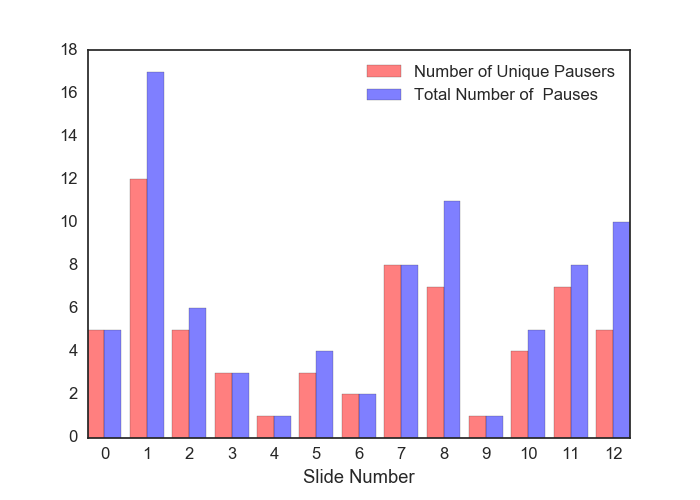
\includegraphics[width=0.4\textwidth]{pictures/pauses.png}
\caption{Pauses}
\label{bintree}
\end{wrapfigure} \\
We decided to use only the number of total pauses. The only problem with this is that the duration of the slide is not taken in account. It means that a very long slide could obtain a much better score than a short one. \\
\\
We've decided not to take in account the duration of slide (also called the time normalization) for a simple reason. The idea behind this project is to identify the problematic parts of a video, meaning the slides without enough explanations, or elements considered as acquired by the teacher while the users do not have them in their knowledge package. The duration of the slide is irrelevant in this case, as the slides are separated in a way that each one only covers one topic. We will compare those results with the ones of the Seek event in a following section.

\subsubsection{Seeks}

\begin{wrapfigure}{l}{0.4\textwidth} %this figure will be at the right
\centering
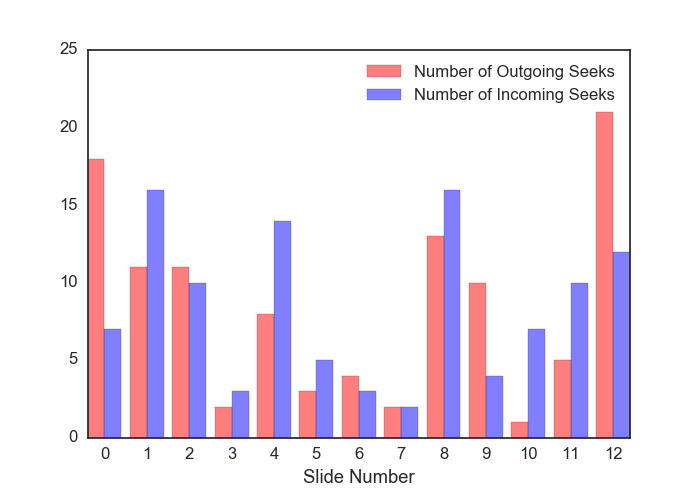
\includegraphics[width=0.4\textwidth]{pictures/seeks.png}
\caption{Seeks}
\label{seeks}
\end{wrapfigure} 

The Seek Data is quite interesting, due to the fact that we have two separate information for each slide, namely the number of users seeking something from this slide, and the number of users seeking this slide. As we can see on figure \ref{seeks}, those two numbers are quite different. At this point we chose to mainly analyze the number of incoming seeks, as the number of people looking for information in a slide is more relevant than the number of people seeking information at this moment. At this point, we could have used only the number of different people seeking a particular slide. We found that a majority of users only seek one time. This is comforting our hypothesis. Users will be more likely to pause and play multiple times inside the same slide, if something is still unclear. If you go backward or forward in time to fetch information, you will obtain it and not going back. Therefore we chose not to take the number of unique seekers.

\subsubsection{Camparison Seeks / Pauses\&Plays}

Now, we want to see if a correlation exists between the total number of pauses and seeks on a same slide. This is shown is figure \ref{comparison}. In order to do that, we normalized the Data, to obtain ratios.
\begin{wrapfigure}{r}{0.5\textwidth} %this figure will be at the right
\centering
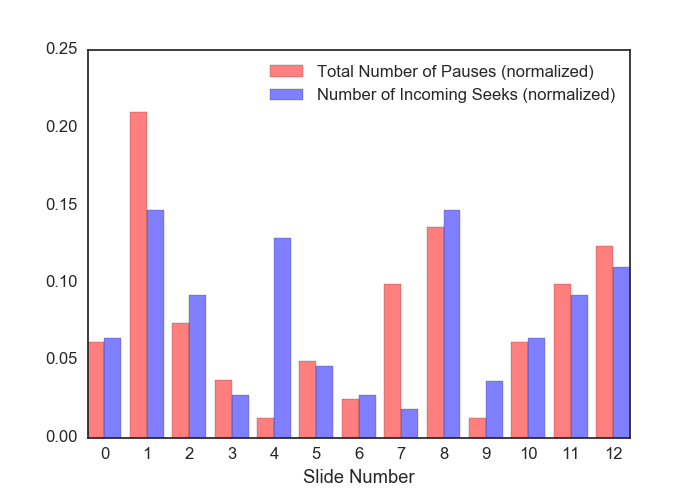
\includegraphics[width=0.5\textwidth]{pictures/comparison.png}
\caption{Comparison}
\label{comparison}
\end{wrapfigure} 
Figure \ref{comparison} shows us interesting things. First, for a large majority of slides, the Data is consistent. Only two slides seem to differ, slide 4 and 7. This is where the usage of a script could be limiting. As human beings, we can check those slides in order to find potential reasons for this difference. \\
Concerning slide 4, the most reasonable explanation is that this slide is the first in a chain of equations, which stay on the same background. Therefore, is a user has problems understanding the entire explanation, he will most likely go back to the beginning (slide 4) in order to listen to the entire explanation. On the contrary, users won't pause the video at this moment, as the explanation just begun. This is consistent with the fact that the number of incoming seeks is way higher than the number of pauses. \\
For slide 7, the explanation is the opposite as slide 4. Slide 7 is the final slide of this explanation. Therefore, users will more likely pause the video at this moment, in order to have all the equations displayed on the background. They won't seek to this specific moment, as the explanation has already been given, and it's hard to understand everything only with the equations. \\
\\
At this point, we chose only to display Data of Seeks and not Pauses\&Plays, as they are almost equivalent. Seeks give the teacher more information, therefore our visualization only shows them.

\section{Visualization}

The goal is to create an intuitive tool for teachers. It needs to be straightforward, understandable and easy to use. In order to achieve that, we've listed the things that should be highlighted. The first look at the page should make the teacher want to play with the tool. Figure \ref{initial} shows the page as it is when you load it.

\subsection{Initial Aspect}
The elements discussed above are present. The slides are represented by the nodes at the bottom, the fact that we are talking about videos is enforced is four different ways. First, the navigation panel on top left has the Course title displayed, then the snapshots of all the slides are displayed in the middle. Third, the big image on top has a progress bar with timer on each side, which refer to a video, and finally the top right panel has a slider called "Auto-play", once again referring to a video.\\
\\
The top right panel also has a slider called "Flowchart". It expands / collapses the flowchart on the bottom. We've decided to add a extra-button on the bottom, between the two rows of nodes, to make the teacher use of of them, as expanding the flowchart is mandatory in order to use the tool in its integrality. \\
\\
In order to keep the teachers focus on the important details, the colors had been reduced to the minimum. We only use two colors, the green and the blue, which are taken from the Google \cite{google} logo. They are well contrasted, and widely used. All the colors displayed on the page are shades of grey, blue or green. The only exception are the snapshots and the video.

\begin{figure}[t]
\captionsetup{justification=centering}
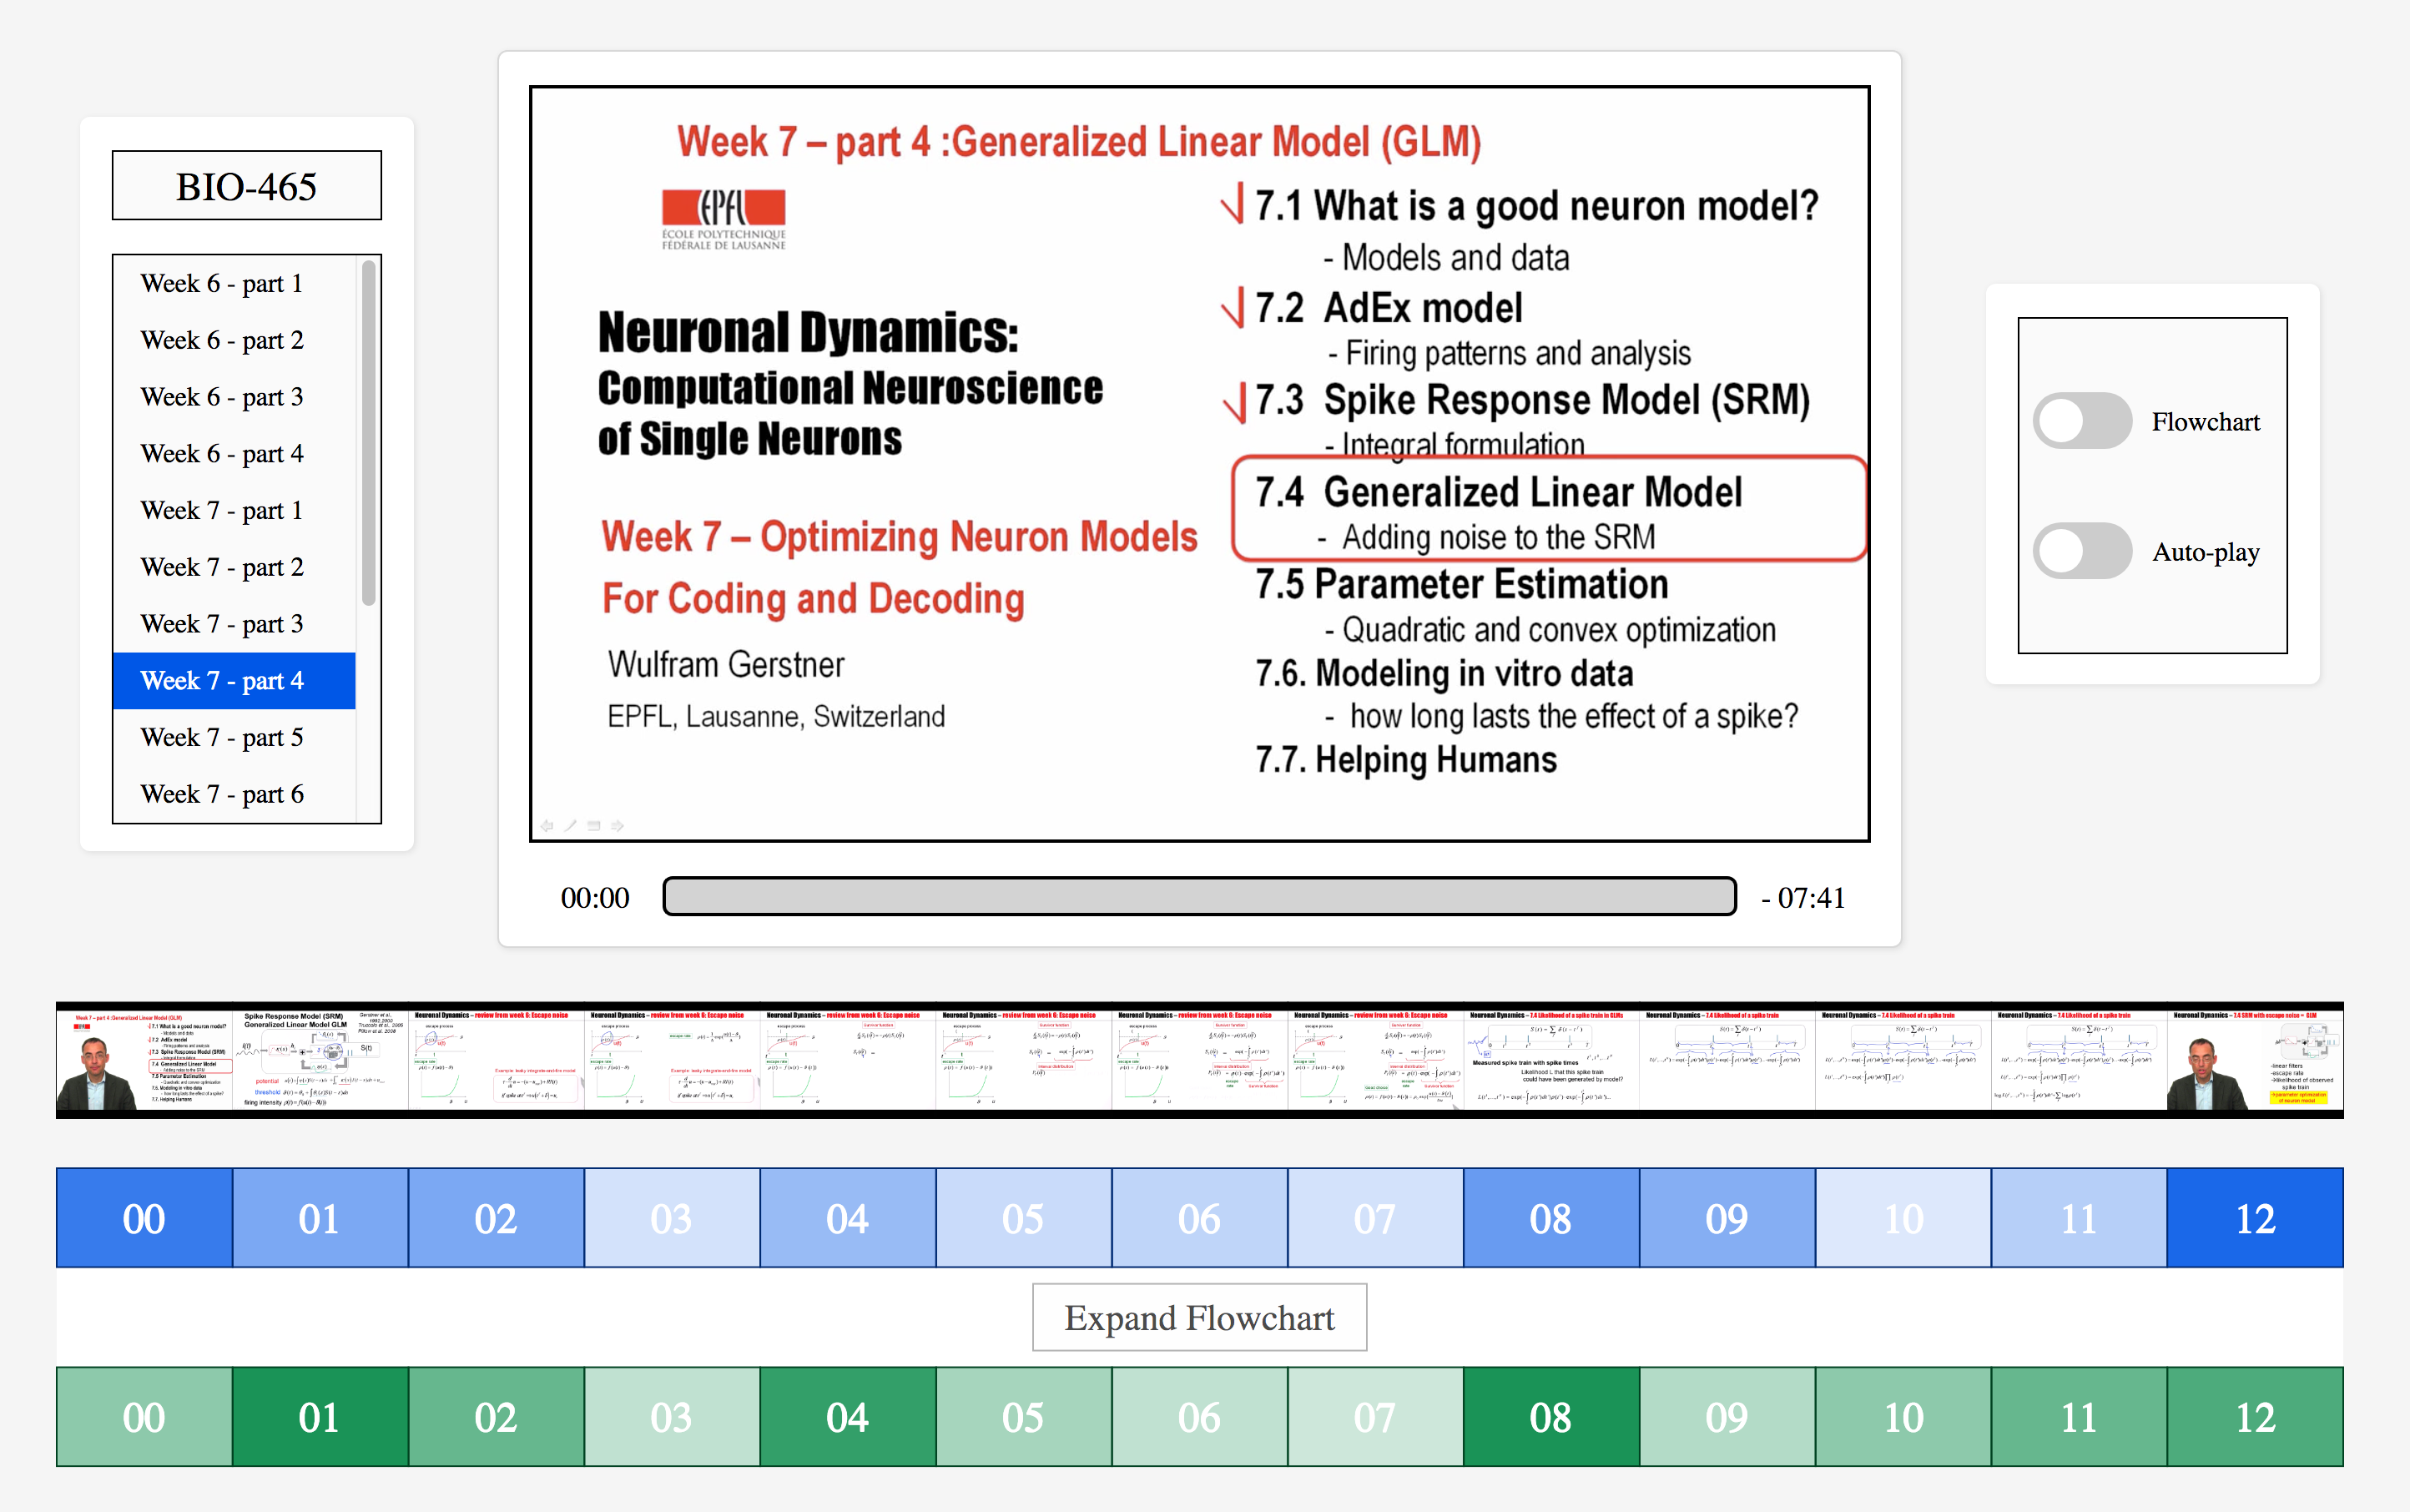
\includegraphics[width=\textwidth]{pictures/initial.png}
\caption{Initial aspect of the page}
\label{initial}
\end{figure} 

\subsection{Expanded Aspect}

Once the teacher has expanded the view via one of the two ways mentioned above, he should play a bit with the flowchart. It has been designed in the most intuitive way possible, allowing the teacher to learn things very quickly, both via the shapes and the colors of the elements displayed. \\
\\
Figure \ref{expanded} shows the page in its expanded state. In the following section, all elements of the page will be explained.

\subsubsection{Elements of the Page}

\begin{figure}[t]
\captionsetup{justification=centering}
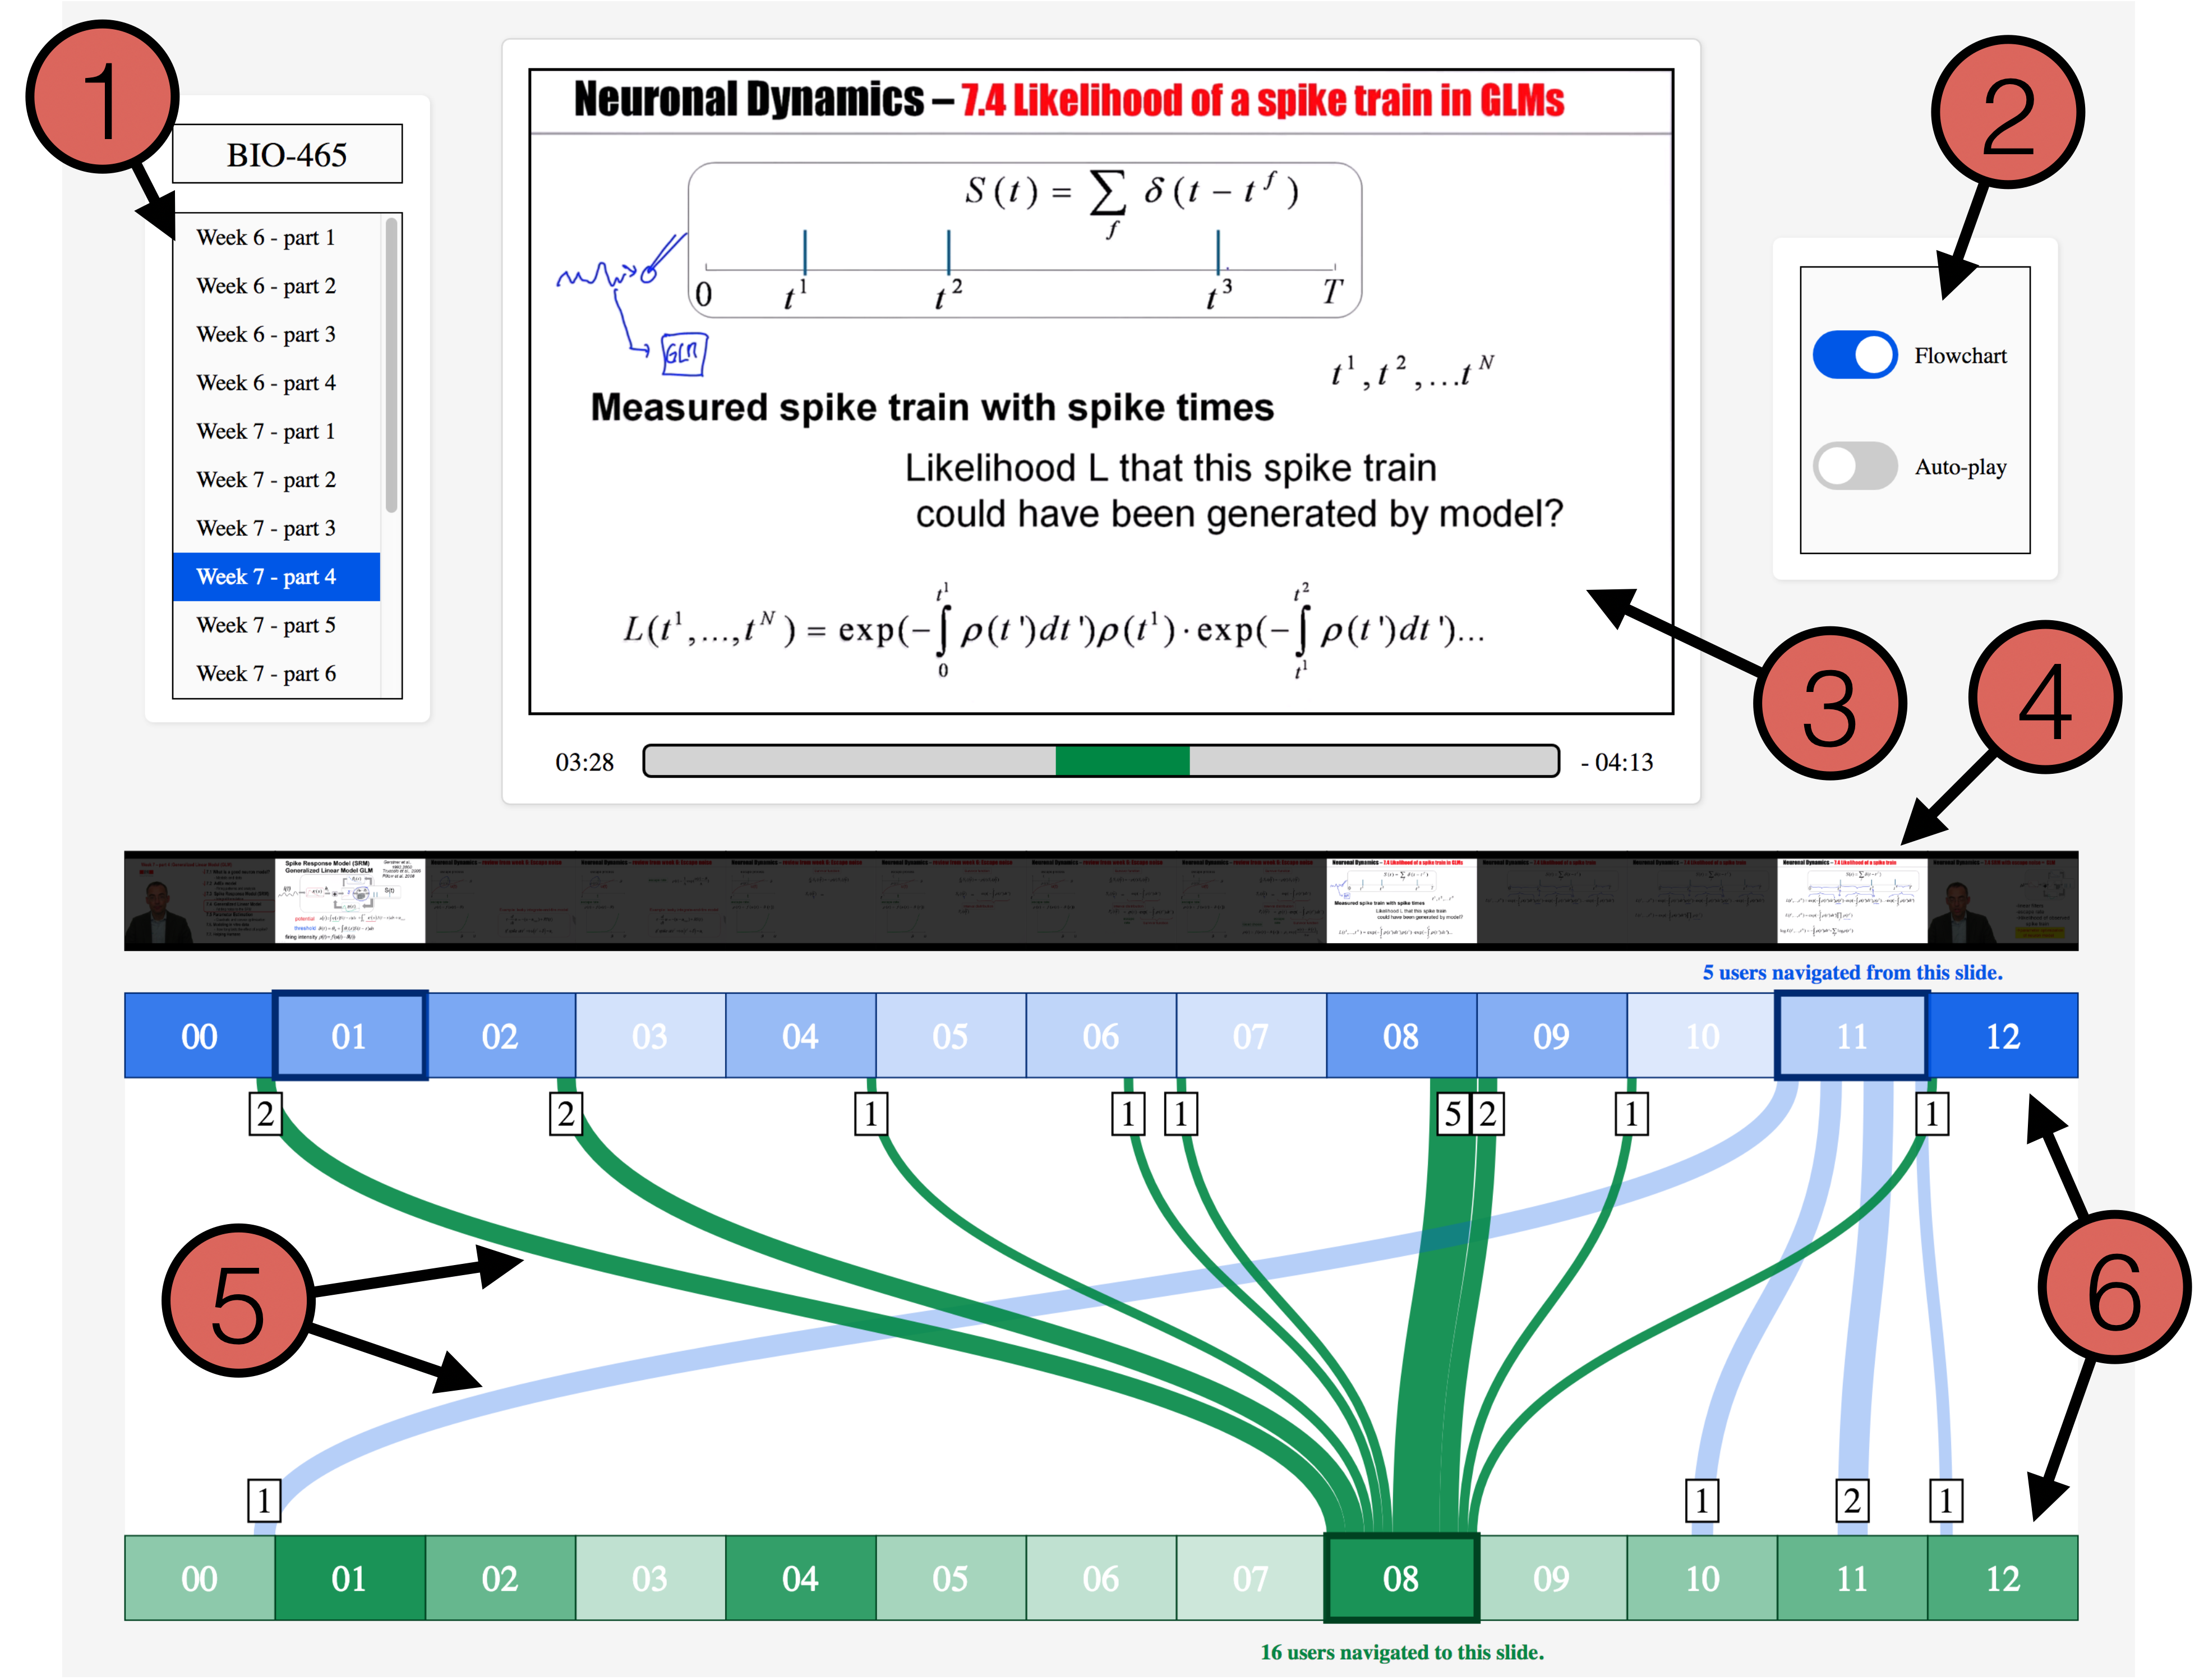
\includegraphics[width=\textwidth]{pictures/expanded_annotated.png}
\caption{Expanded aspect of the page}
\label{expanded}
\end{figure} 

\begin{enumerate}
    \item The top left panel is the video browser. As mentioned above, the color used for the selected video is the same blue as in all the page. The description of each video is simplified as much as possible. We also put the code of the Course as a title. The teacher will know which course it is, as they do not have that much different courses to teach. Putting only the code adds clarity to the page. \\
    When the teacher clicks on one video, the entire tool is refreshed, displaying the Data of the new video.
    \item The top right panel only contains two elements. Those two sliders have a simple word as label, to avoid overwhelming the users with too much text. The first one controls the expansion of the flowchart, as explained in the previous section. The second one is called "Auto-play". It controls the content of element (3), which is the video in the middle. One could think that the video is always displayed on the top, and will play automatically. This is indeed the default behaviour of the tool. We've added a simple functionality, which will allow the teacher to display only the snapshot of each slide, instead of playing the video. This could be useful at the beginning for example, when the teacher wants to remember the exact content of its Course. Once it is clear for him, he can just switch back to auto-play, and then video will start automatically when he selects a slide.
    \item The video is the more important element of the page. This is where the teacher will make the connection between the Data shown in the flowchart, and the video itself. As explained above, the big image displays either the video, or a simple snapshot of a slide. The problem we had with this implementation is that the duration / time location of the slide were not represented. The progress bar below the image shows those two things. the highlighted part represents the time location of the slide, inside the video. At each extremity, there is a time. The left one represents the elapsed time, while the right one represents the remaining time. The teacher will have the exact timing of the slide along with a visual representation of the duration of the slide, compared to the duration of the entire video. The highlighted part is filled with green or blue, depending on the class of the selected node (source or target).
    \item The snapshots bar has a single purpose. When no slide is selected, all the snapshots are visible. It gives the teacher the opportunity to find visually a slide he knows, or a slide he wants to know more about, for example. If the teacher only mouse-over a node, only the corresponding slide will stay visible, all the other ones will be greyed. The corresponding content will also be displayed in the top frame, either as a snapshot or the video depending on the state of the Auto-play slider. As you can see on the screen, if the teacher has selected more than one node, all the corresponding snapshots will stay visible.
    \item The links are the core of the flowchart. The idea behind this flowchart is to regroup in one place all the information we have from the Seek Data. For each slide, we have the number of users going to every slide from this one, and coming from every slide to this one. Therefore, each slide acts both as source and as target. We've represented each slide as a node, present twice (as source and target). To stay in our color code, the green means target, therefore all links going to the selected target will be green, as well as the node itself. Those links have a thickness representing the number of users who travelled from a specific slide to another one. This number is also written in a small square box, in order for the teacher to have all the information we can give him displayed as intuitively as possible.
    \item Finally, the rectangles represent the slides. As mentioned above, the blue means source, and the green target. The flowchart goes downward, thus the top row represents the sources while the bottom one represents the targets. In order to display the information about the importance of each slide while keeping the color code of only one color per class, we had to use opacity. For each class, the slide with the highest number of incoming/outgoing links is displayed with the maximum opacity (in our example, source n°12 and target n°8). All the other slides have an opacity linearly decreasing with their importance. This way, the flowchart displays everything we have while only using 2 colors. 
\end{enumerate}

\section{Conclusion}

The goal of this project has been reached, but not entirely. The initial idea was to create a tool which allows every MOOC teacher to have an instant feedback on his Courses. The problem is that we did not have enough time to work on a slide detection script, which would have automatized the entire process. For now, we still have to do it manually. Once the time stamps of the slide changes are calculated, our script creates the JSON file which fits in the tool directly, therefore we don't have more than one intermediate step. \\
\\
The second problem is that, initially, we wanted to have a global grid representing all the videos of all the courses. The teacher should have been able to select his courses from there, and then to have access to our tool. This first layout of the tool is still undone, unfortunately.\\
\\
Overall, this project has been a very good experience. The fact that we did some Data analysis and some visualization is a big plus. I hope my work will be continued by someone else. The teachers deserve to have a real tool for the MOOCs. 

\begin{thebibliography}{1}

\bibitem{coursera}
Coursera : https://www.coursera.org

\bibitem{edx}
EDX : https://www.edx.org

\bibitem{google}
Google : https://www.google.com
\end{thebibliography}

\end{document}

